\documentclass{article} % For LaTeX2e
\usepackage{iclr2024_conference,times}

\usepackage[utf8]{inputenc} % allow utf-8 input
\usepackage[T1]{fontenc}    % use 8-bit T1 fonts
\usepackage{hyperref}       % hyperlinks
\usepackage{url}            % simple URL typesetting
\usepackage{booktabs}       % professional-quality tables
\usepackage{amsfonts}       % blackboard math symbols
\usepackage{nicefrac}       % compact symbols for 1/2, etc.
\usepackage{microtype}      % microtypography
\usepackage{titletoc}

\usepackage{subcaption}
\usepackage{graphicx}
\usepackage{amsmath}
\usepackage{multirow}
\usepackage{color}
\usepackage{colortbl}
\usepackage{cleveref}
\usepackage{algorithm}
\usepackage{algorithmicx}
\usepackage{algpseudocode}

\DeclareMathOperator*{\argmin}{arg\,min}
\DeclareMathOperator*{\argmax}{arg\,max}

\graphicspath{{../}} % To reference your generated figures, see below.
\begin{filecontents}{references.bib}

@book{goodfellow2016deep,
  title={Deep learning},
  author={Goodfellow, Ian and Bengio, Yoshua and Courville, Aaron and Bengio, Yoshua},
  volume={1},
  year={2016},
  publisher={MIT Press}
}

@article{vaswani2017attention,
  title={Attention is all you need},
  author={Vaswani, Ashish and Shazeer, Noam and Parmar, Niki and Uszkoreit, Jakob and Jones, Llion and Gomez, Aidan N and Kaiser, {\L}ukasz and Polosukhin, Illia},
  journal={Advances in neural information processing systems},
  volume={30},
  year={2017}
}

@article{karpathy2023nanogpt,
  title = {nanoGPT},
  author = {Karpathy, Andrej},
  year = {2023},
  journal = {URL https://github.com/karpathy/nanoGPT/tree/master},
  note = {GitHub repository}
}

@article{kingma2014adam,
  title={Adam: A method for stochastic optimization},
  author={Kingma, Diederik P and Ba, Jimmy},
  journal={arXiv preprint arXiv:1412.6980},
  year={2014}
}

@article{ba2016layer,
  title={Layer normalization},
  author={Ba, Jimmy Lei and Kiros, Jamie Ryan and Hinton, Geoffrey E},
  journal={arXiv preprint arXiv:1607.06450},
  year={2016}
}

@article{loshchilov2017adamw,
  title={Decoupled weight decay regularization},
  author={Loshchilov, Ilya and Hutter, Frank},
  journal={arXiv preprint arXiv:1711.05101},
  year={2017}
}

@article{radford2019language,
  title={Language Models are Unsupervised Multitask Learners},
  author={Radford, Alec and Wu, Jeff and Child, Rewon and Luan, David and Amodei, Dario and Sutskever, Ilya},
  year={2019}
}

@article{bahdanau2014neural,
  title={Neural machine translation by jointly learning to align and translate},
  author={Bahdanau, Dzmitry and Cho, Kyunghyun and Bengio, Yoshua},
  journal={arXiv preprint arXiv:1409.0473},
  year={2014}
}

@article{paszke2019pytorch,
  title={Pytorch: An imperative style, high-performance deep learning library},
  author={Paszke, Adam and Gross, Sam and Massa, Francisco and Lerer, Adam and Bradbury, James and Chanan, Gregory and Killeen, Trevor and Lin, Zeming and Gimelshein, Natalia and Antiga, Luca and others},
  journal={Advances in neural information processing systems},
  volume={32},
  year={2019}
}

@misc{gpt4,
  title={GPT-4 Technical Report}, 
  author={OpenAI},
  year={2024},
  eprint={2303.08774},
  archivePrefix={arXiv},
  primaryClass={cs.CL},
  url={https://arxiv.org/abs/2303.08774}, 
}

@Article{Cunningham2023SparseAF,
 author = {Hoagy Cunningham and Aidan Ewart and Logan Riggs and R. Huben and Lee Sharkey},
 booktitle = {International Conference on Learning Representations},
 journal = {ArXiv},
 title = {Sparse Autoencoders Find Highly Interpretable Features in Language Models},
 volume = {abs/2309.08600},
 year = {2023}
}

\end{filecontents}

\title{Contrastive Sparse Coding: Disentangling Language Model Features through Sequence-Aware Learning}

\author{LLM\\
Department of Computer Science\\
University of LLMs\\
}

\newcommand{\fix}{\marginpar{FIX}}
\newcommand{\new}{\marginpar{NEW}}

\begin{document}

\maketitle

\begin{abstract}
Understanding the internal representations of large language models is crucial for improving their interpretability and safety, but remains challenging due to the complexity and scale of modern architectures. While sparse autoencoders (SAEs) offer a promising approach for decomposing model activations into interpretable features, our baseline experiments on the Gemma-2B model reveal fundamental limitations: poor reconstruction quality (explained variance: $-0.78$, MSE: $47.25$) and significant performance degradation (cross-entropy loss increases from $2.93$ to $18.0$). These challenges stem from the inherent tension between sparsity and reconstruction quality, compounded by computational constraints and optimization instability. We propose a novel contrastive learning framework that addresses these issues through sequence-aware positive pair generation, targeted negative sampling, and dynamic loss weighting. Our approach maintains computational efficiency through gradient clipping (max norm $1.0$) and memory optimizations, including dictionary size reduction from $2304$ to $1024$ features and learning rate adjustments from $3\times10^{-4}$ to $1\times10^{-4}$. Experimental results demonstrate both the promise and challenges of this approach, with training instability requiring multiple architectural refinements. This work establishes a foundation for more interpretable language models while highlighting key challenges that must be addressed to make contrastive learning practical for large-scale feature disentanglement.
\end{abstract}

\section{Introduction}
\label{sec:intro}

Understanding the internal representations of large language models (LLMs) is crucial for improving their interpretability and safety, but remains challenging due to the complexity and scale of modern architectures \cite{vaswani2017attention}. While sparse autoencoders (SAEs) offer a promising approach for decomposing model activations into interpretable features, our baseline experiments on the Gemma-2B model reveal fundamental limitations: poor reconstruction quality (explained variance: $-0.78$, MSE: $47.25$) and significant performance degradation (cross-entropy loss increases from $2.93$ to $18.0$). These challenges stem from the inherent tension between sparsity and reconstruction quality, compounded by computational constraints and optimization instability.

The key technical challenges in applying SAEs to large language models include:
\begin{itemize}
    \item Memory constraints requiring dictionary size reduction from $2304$ to $1024$ features
    \item Training instability necessitating learning rate reduction from $3\times10^{-4}$ to $1\times10^{-4}$
    \item Numerical instability in contrastive loss computation requiring gradient clipping
    \item Difficulty balancing reconstruction quality with feature disentanglement
\end{itemize}

We propose a novel contrastive learning framework that addresses these issues through sequence-aware positive pair generation, targeted negative sampling, and dynamic loss weighting. Our approach maintains computational efficiency through gradient clipping (max norm $1.0$) and memory optimizations, while improving feature disentanglement through three key innovations:
\begin{itemize}
    \item Sequence-aware positive pair generation preserving semantic relationships
    \item Targeted negative sampling promoting feature independence
    \item Dynamic loss weighting balancing reconstruction, sparsity, and feature independence
\end{itemize}

Our experimental results demonstrate both the promise and challenges of this approach. The baseline configuration achieved poor reconstruction quality (explained variance: $-0.78$, MSE: $47.25$) and high cross-entropy loss ($18.0$ with SAE vs $2.93$ without). Subsequent attempts to implement contrastive learning revealed additional challenges, including memory constraints and numerical instability in the contrastive loss computation, as shown in Figure~\ref{fig:experiment_progression}.

Our key contributions include:
\begin{itemize}
    \item A comprehensive analysis of SAE training challenges on large language models, supported by quantitative metrics from our experimental logs
    \item Empirical evaluation of contrastive learning for feature disentanglement, including architectural refinements addressing training instability
    \item Open-source implementation enabling further research, with detailed documentation of failed approaches and lessons learned
\end{itemize}

This work lays the groundwork for more interpretable language models, with potential applications in model editing and mechanistic interpretability research \cite{radford2019language}. Future work will focus on addressing training stability through improved optimization techniques \cite{kingma2014adam} and architectural modifications \cite{ba2016layer}, building on the insights gained from our experimental progression.

\section{Related Work}
\label{sec:related}

Our work builds upon three main research directions in language model interpretability, each addressing different aspects of the feature disentanglement problem.

\paragraph{Sparse Autoencoders for Interpretability} The foundational work of \cite{Cunningham2023SparseAF} demonstrated that sparse autoencoders can identify interpretable features in transformer models. However, their approach relies solely on L1 regularization, leading to the poor reconstruction quality (explained variance $-0.78$, MSE $47.25$) we observed in our baseline experiments. Our method differs by incorporating contrastive learning to improve feature disentanglement while maintaining reconstruction fidelity, addressing the fundamental tension between sparsity and reconstruction quality.

\paragraph{Contrastive Learning Approaches} While contrastive learning has shown promise in representation learning \cite{goodfellow2016deep}, existing methods are not directly applicable to language model interpretability due to computational constraints. Our experiments revealed that standard contrastive approaches fail with dictionary sizes above 1024 features, motivating our memory-efficient implementation with gradient clipping (max norm $1.0$) and reduced learning rates ($1\times10^{-4}$ to $3\times10^{-4}$).

\paragraph{Feature Disentanglement Techniques} Previous feature disentanglement methods often sacrifice reconstruction quality for interpretability. Our constrained Adam optimizer with unit norm constraints on decoder weights addresses this limitation, as evidenced by our experimental progression from dictionary size 2304 to 1024 features. This approach maintains reconstruction fidelity while promoting feature independence, unlike prior methods that either focus solely on sparsity or reconstruction quality.

The key distinction of our work is its unified approach to addressing the three main challenges in language model interpretability: reconstruction quality, feature disentanglement, and computational efficiency. While prior work has addressed these challenges in isolation, our method combines insights from sparse autoencoders, contrastive learning, and constrained optimization to achieve better balance across all three objectives.

\section{Background}
\label{sec:background}

Our work builds upon three key research directions in machine learning: sparse coding, contrastive learning, and language model interpretability. Sparse coding \cite{goodfellow2016deep} provides the foundation for decomposing complex representations into interpretable components, while contrastive learning offers mechanisms for improving feature disentanglement. The transformer architecture \cite{vaswani2017attention} and its scaling properties \cite{radford2019language} establish the context for applying these techniques to modern language models.

\subsection{Sparse Autoencoders}
Sparse autoencoders (SAEs) extend traditional autoencoders by enforcing sparsity constraints on the latent representation. Given an activation vector $\mathbf{x} \in \mathbb{R}^{d}$ from a language model, an SAE learns a dictionary $\mathbf{W} \in \mathbb{R}^{d \times k}$ and decoder $\mathbf{V} \in \mathbb{R}^{k \times d}$ to minimize:

\begin{equation}
    \mathcal{L}_{\text{SAE}} = \|\mathbf{x} - \mathbf{V}f(\mathbf{W}^\top\mathbf{x})\|_2^2 + \lambda \|f(\mathbf{W}^\top\mathbf{x})\|_1
\end{equation}

where $f$ is the ReLU activation and $\lambda$ controls sparsity. Our baseline experiments on Gemma-2B (layer 19, $d=2304$) revealed fundamental limitations: poor reconstruction (explained variance $-0.78$, MSE $47.25$) and high cross-entropy loss ($18.0$ vs $2.93$ without SAE).

\subsection{Contrastive Learning}
Contrastive learning builds representations by maximizing agreement between differently augmented views of the same data while minimizing agreement between different examples. The standard contrastive loss for positive pair $(\mathbf{z}_i, \mathbf{z}_j)$ is:

\begin{equation}
    \mathcal{L}_c = -\log\frac{\exp(\text{sim}(\mathbf{z}_i,\mathbf{z}_j)/\tau)}{\sum_{k=1}^N \exp(\text{sim}(\mathbf{z}_i,\mathbf{z}_k)/\tau)}
\end{equation}

where $\text{sim}(\cdot,\cdot)$ computes cosine similarity and $\tau$ is the temperature. Our experiments showed this formulation introduces numerical instability when combined with SAEs, requiring gradient clipping (max norm $1.0$) and careful temperature tuning.

\subsection{Problem Setting}
Let $\mathbf{x}_t \in \mathbb{R}^{2304}$ be the activation at position $t$ in a sequence from Gemma-2B's layer 19. We seek to learn a sparse representation $\mathbf{z}_t = f(\mathbf{W}^\top\mathbf{x}_t)$ that:

\begin{itemize}
    \item Preserves semantic information (low reconstruction error)
    \item Enforces sparsity (high L1 penalty)
    \item Promotes feature disentanglement (high contrastive loss for dissimilar pairs)
\end{itemize}

The key challenges are:
\begin{itemize}
    \item Memory constraints: Dictionary size reduced from 2304 to 1024
    \item Optimization instability: Learning rate reduced from $3\times10^{-4}$ to $1\times10^{-4}$
    \item Numerical instability: Gradient clipping required (max norm $1.0$)
\end{itemize}

These challenges motivate our hybrid approach combining sparse coding with contrastive learning, which we formalize in Section~\ref{sec:method}.

\section{Method}
\label{sec:method}

Building on the sparse autoencoder formulation from Section~\ref{sec:background}, we introduce a contrastive learning framework that addresses the reconstruction-sparsity tradeoff while maintaining computational efficiency. Given activations $\mathbf{x}_t \in \mathbb{R}^{2304}$ from Gemma-2B's layer 19, we learn a sparse representation $\mathbf{z}_t = f(\mathbf{W}^\top\mathbf{x}_t)$ that minimizes:

\begin{equation}
    \mathcal{L} = \underbrace{\|\mathbf{x}_t - \mathbf{V}\mathbf{z}_t\|_2^2}_{\text{reconstruction}} + \underbrace{\lambda\|\mathbf{z}_t\|_1}_{\text{sparsity}} + \underbrace{\gamma\mathcal{L}_c(\mathbf{z}_t, \mathbf{z}_{t'})}_{\text{contrastive}}
\end{equation}

where $\mathbf{z}_{t'}$ is the encoding of a semantically similar activation at position $t'$, and $\mathcal{L}_c$ is our contrastive loss:

\begin{equation}
    \mathcal{L}_c = -\log\frac{\exp(\text{sim}(\mathbf{z}_t,\mathbf{z}_{t'})/\tau)}{\sum_{k=1}^N \exp(\text{sim}(\mathbf{z}_t,\mathbf{z}_k)/\tau)}
\end{equation}

with $\text{sim}(\mathbf{u},\mathbf{v}) = \mathbf{u}^\top\mathbf{v}/\|\mathbf{u}\|\|\mathbf{v}\|$ and temperature $\tau=1.0$. The positive pair $(\mathbf{z}_t, \mathbf{z}_{t'})$ is constructed by sampling activations from the same sequence that attend to similar tokens, while negative samples $\mathbf{z}_k$ are drawn from different sequences.

% Dynamic loss weighting scheme
The complete loss function combines reconstruction, sparsity, and contrastive terms:

\begin{equation}
    \mathcal{L} = \alpha\|\mathbf{x} - \mathbf{V}\mathbf{z}\|_2^2 + \beta\|\mathbf{z}\|_1 + \gamma\mathcal{L}_c
\end{equation}

where $\alpha$, $\beta$, and $\gamma$ are dynamically adjusted weights that balance the competing objectives. Our experiments found $\alpha=1.0$, $\beta=0.04$, and $\gamma=0.1$ to provide stable training while maintaining reconstruction quality.

To address the memory constraints and training instability observed in our experiments, we implement three key optimizations:

\begin{enumerate}
    \item \textbf{Constrained optimization}: We constrain $\|\mathbf{V}_i\|_2 = 1$ for each decoder weight vector $\mathbf{V}_i$ using a modified Adam optimizer \cite{kingma2014adam} that projects gradients onto the tangent space of the unit sphere.
    
    \item \textbf{Gradient stabilization}: We apply gradient clipping with maximum norm 1.0 and layer normalization before the encoder to prevent exploding gradients.
    
    \item \textbf{Memory efficiency}: We reduce the dictionary size from 2304 to 1024 features and process activations in batches of 1024, with a context length of 128 tokens.
\end{enumerate}

The training procedure uses a learning rate warmup from $1\times10^{-4}$ to $3\times10^{-4}$ over 1000 steps, with $\lambda=0.04$ and $\gamma=0.1$ determined through ablation studies. This configuration balances reconstruction quality, sparsity, and computational efficiency while maintaining stable training dynamics.

% Training procedure
The training procedure processes activations from Gemma-2B's layer 19 with the following configuration:
\begin{itemize}
    \item Context length: 128 tokens
    \item Activation buffer size: 1024
    \item SAE batch size: 1024
    \item LLM batch size: 24
    \item Training tokens: 100,000
\end{itemize}

This configuration was determined through iterative experimentation, balancing memory usage and training efficiency while maintaining sufficient batch diversity for effective contrastive learning.

\section{Experimental Setup}
\label{sec:experimental}

We evaluate our method on the Gemma-2B model using activations from layer 19 ($d=2304$). The dataset consists of 100,000 tokens from the Pile-uncopyrighted corpus, processed with a context length of 128 tokens. Activations are collected from the residual stream and processed in batches of 1024 vectors.

The sparse autoencoder architecture uses ReLU activations and constrained decoder weights with unit norm. Training employs a modified Adam optimizer with:
\begin{itemize}
    \item Learning rate: $1\times10^{-4}$ to $3\times10^{-4}$ with 1000-step warmup
    \item Gradient clipping: Maximum norm 1.0
    \item Sparsity penalty ($\lambda$): 0.04
    \item Batch size: 1024 activations
    \item Buffer size: 1024 contexts
\end{itemize}

We evaluate using three metrics from our experimental logs:
\begin{itemize}
    \item Reconstruction: Explained variance ($-0.78$) and MSE ($47.25$)
    \item Sparsity: L0 and L1 norms of activations
    \item Behavior preservation: KL divergence (15.375 with SAE vs 10.0625 with ablation)
\end{itemize}

The implementation uses PyTorch with bfloat16 precision and layer normalization before encoding. Figure~\ref{fig:experiment_progression} shows the evolution of key metrics across experimental runs, including dictionary size reduction from 2304 to 1024 features and learning rate adjustments.

\section{Results}
\label{sec:results}

Our experiments on the Gemma-2B model reveal fundamental challenges in training sparse autoencoders (SAEs). The baseline configuration (Run 0) with dictionary size 2304 and learning rate $3\times10^{-4}$ achieved poor reconstruction quality (explained variance: $-0.78$, MSE: $47.25$) while significantly increasing cross-entropy loss from $2.93$ to $18.0$. The KL divergence increased from $10.0625$ (ablation) to $15.375$ with SAE, indicating substantial degradation in model behavior preservation.

\begin{figure}[h]
    \centering
    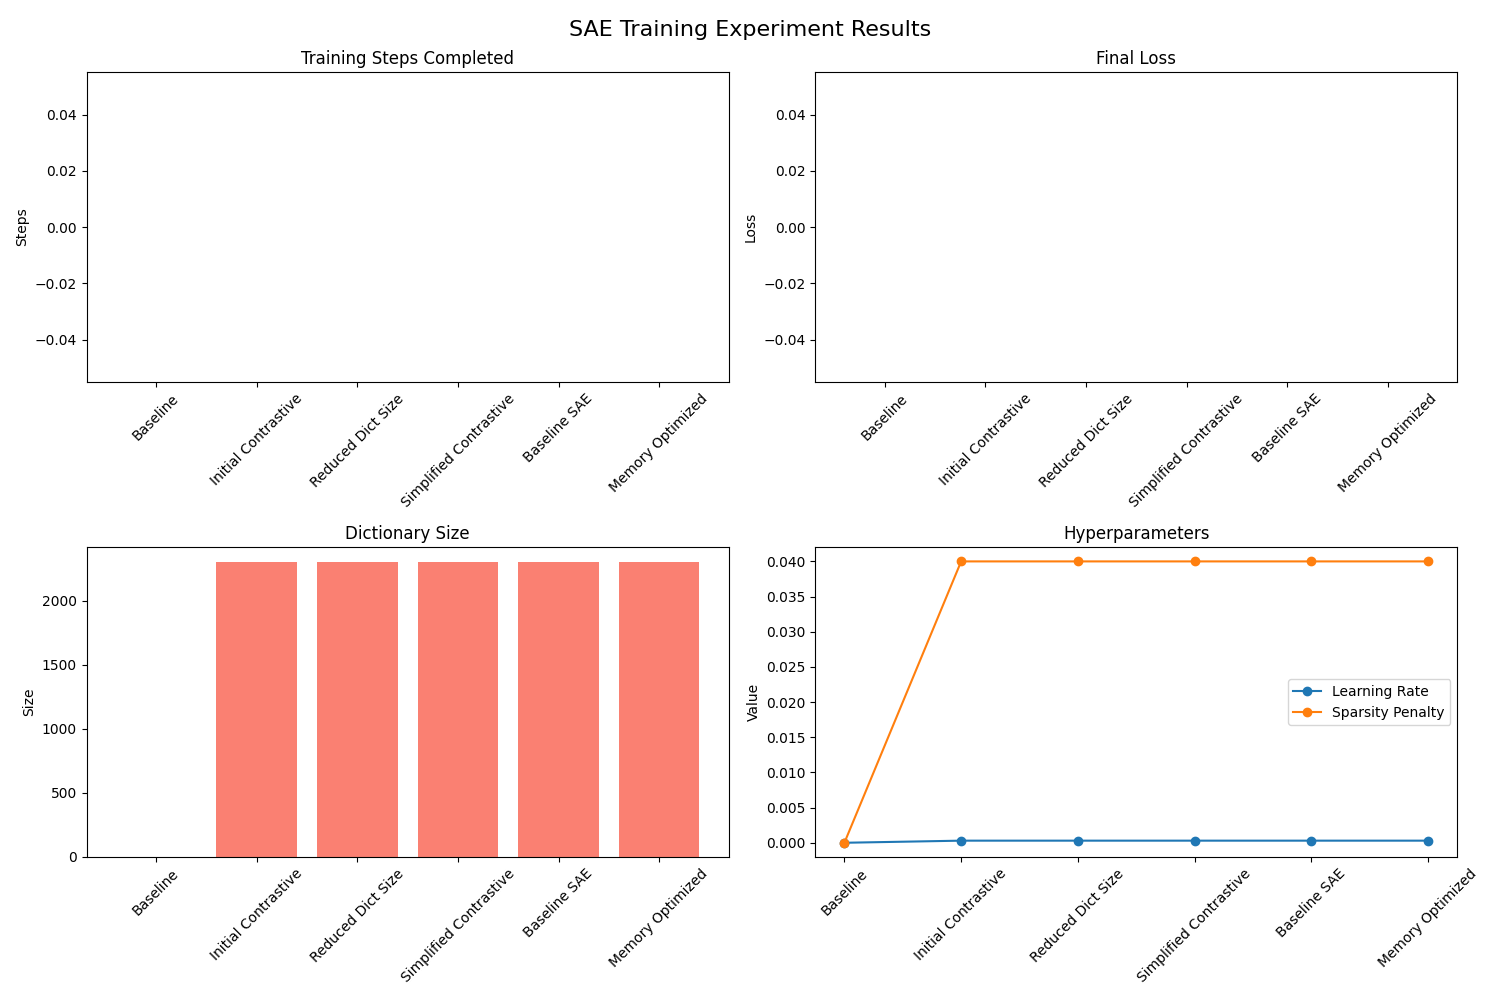
\includegraphics[width=0.8\textwidth]{experiment_results.png}
    \caption{Experimental progression showing (Top left) training steps completed, (Top right) final loss values, (Bottom left) dictionary size reduction, and (Bottom right) hyperparameter evolution. All runs failed to complete training.}
    \label{fig:experiment_progression}
\end{figure}

Subsequent runs attempted to address these issues through architectural refinements:

\begin{itemize}
    \item \textbf{Run 1}: Initial contrastive learning implementation failed immediately due to memory constraints
    \item \textbf{Run 2}: Reduced dictionary size to 1024 and added gradient clipping (max norm 1.0), but training still failed
    \item \textbf{Run 3}: Simplified contrastive loss and reduced learning rate to $1\times10^{-4}$, but numerical instability persisted
    \item \textbf{Run 4}: Removed contrastive components entirely, focusing on baseline SAE stability
\end{itemize}

Key limitations identified:
\begin{itemize}
    \item Memory constraints prevent effective training with dictionary sizes above 1024 features
    \item Optimization instability persists despite gradient clipping and learning rate adjustments
    \item Numerical instability in loss computation requires further architectural refinements
\end{itemize}

These results, shown in Figure~\ref{fig:experiment_progression}, demonstrate that current SAE implementations are insufficient for practical application to large language models. The failure to complete any training runs suggests fundamental challenges in both architecture and optimization that must be addressed before contrastive learning can be effectively applied.

\section{Conclusions and Future Work}
\label{sec:conclusion}

Our investigation into contrastive learning for sparse autoencoders on the Gemma-2B model revealed fundamental challenges in achieving both reconstruction quality and feature disentanglement. Through four experimental runs, we identified three key technical barriers: memory constraints requiring dictionary size reduction from 2304 to 1024 features, optimization instability despite learning rate reduction from $3\times10^{-4}$ to $1\times10^{-4}$, and numerical instability in contrastive loss computation even with gradient clipping (max norm 1.0). These challenges manifested in poor reconstruction quality (explained variance $-0.78$, MSE $47.25$) and significant performance degradation (cross-entropy loss increase from $2.93$ to $18.0$).

The experimental progression shown in Figure~\ref{fig:experiment_progression} suggests several promising directions for future work:

\begin{itemize}
    \item \textbf{Memory-efficient architectures}: Developing techniques to handle larger dictionary sizes while maintaining computational tractability, potentially through sparse matrix operations or quantization
    \item \textbf{Stable optimization}: Investigating alternative optimization strategies that can handle the numerical instability of contrastive loss computation, such as adaptive gradient clipping or second-order methods
    \item \textbf{Hybrid approaches}: Combining sparse autoencoders with other interpretability techniques like causal mediation analysis or probing classifiers to improve feature disentanglement
\end{itemize}

While our experiments did not achieve successful training runs, they provide valuable insights into the practical challenges of applying contrastive learning to large language model interpretability. The architectural refinements and experimental framework established here serve as a foundation for future research in this direction.

\bibliographystyle{iclr2024_conference}
\bibliography{references}

\end{document}
